\chapter{Implementación y Experimentos} 
\label{sec:Implementacion}
\section{Detalles Técnicos de Implementación} 
Este proyecto ha sido realizado mayoritariamente con el lenguaje de programación Python, 
debido a que casi todos los modelos analizados estaban descritos en el mismo.
No obstante, para la distorsión por compresión \emph{octree}\cite{OctreeCompression}, 
se hizo uso de la librería PCL\cite{PCL} en el lenguaje C++.

Para el desarrollo y ejecución de los modelos fue necesario el uso de librería 
la librería de DL Pytorch junto con las librerías CUDA de para poder ejecutar 
los modelos en las tarjetas gráficas de NVIDIA. Para los cálculos numéricos y 
el manejo de datos se utilizaron Numpy y Polars, librería similar a Pandas 
pero basada en Rust, más eficiente y fácilmente paralelizable. Además, para el
cálculo de las métricas se utilizó la librería scikit-learn.
Para la visualización y fácil manipulación de las nubes de puntos se hizo uso 
de la librería de Open3D\cite{Open3D} y Pyntcloud.
Se ha gestionado el uso de estas librerías y todas sus dependencias tanto en entornos virtuales 
de python como en entornos creados por cuadernos jupyter de Colab.

Para el control de versiones del proyecto se utilizó de forma conjunta Git, GitHub
y la gestión de versiones de Google Drive. El repositorio de este proyecto se 
puede acceder por la siguiente dirección: \url{https://github.com/CodeBoy-source/TFG_NRPCQA}.
Este mismo, se encuentra dividido en un conjunto de carpetas: 
\begin{itemize}
  \item \textbf{Distort}, donde se encuentra todo lo necesario para la generación 
    de las distorsiones médicas dado un directorio de archivos \code{.ply}. 
    A su vez, posee lo necesario para la generación de las etiquetas sintéticas 
    de calidad, ver Sección \ref{sec:DatosSinteticos}.
  \item \textbf{Document}, donde se encuentra la documentación del proyecto, 
    incluyendo a este documento. 
  \item \textbf{NR3DQA}, implementación y experimentos del método propuesto 
    por Zhang et al\cite{NR3DQA}.
  \item \textbf{Utils}, conjunto de scripts de python para la realización de distintas 
    tareas. Como por ejemplo la lectura de un directorio DICOM, la visualización 
    de una o un conjunto de nubes de puntos y división del conjunto de datos LS-SJTU-PCQA\cite{ResSCNN}.
  \item \textbf{VQA\_PC}, implementación de la variante VQA-PC\cite{VQA-PC} para 
    la estimación de calidad de nubes de puntos y las modificaciones pertinentes 
    sobre los métodos de fusión de características mencionados en \cite{EnsemblePCQA}. 
\end{itemize}
\subsection{Obtención de los modelos 3D}
Los datos se encuentran en una carpeta del servicio UGRDrive, que provee almacenamiento 
en la nube para investigadores. Los modelos mencionados en la Sección \ref{sec:OurData} 
se encuentran dentro de una carpeta numerada por cada individuo con los ficheros 
necesarios para el desarrollo del proyecto. Se incluyen incluso algunos directorios 
DICOM enteros por si fuera necesario generar más datos a partir de la segmentación 
manual. 

Se desarrolló un fichero \code{gen_distortions.py} que automáticamente genera 
un conjunto de distorsiones dado un directorio de entrada con archivos \code{.ply} y los 
guarda en un directorio de salida especificado por argumento. Para ello se hace 
uso de las distorsiones realizadas con Open3D\cite{Open3D} 
con el archivo del directorio \code{utils/distortions.py} y un ejecutable hecho 
con C++ y Makefile para la distorsión \emph{octree}. A continuación, 
podemos generar las etiquetas sintéticas con \code{get_metrics.py}, que dado un 
directorio de entrada con las nubes de referencia y uno con las distorsiones, 
genera un \code{.csv} con las etiquetas sintéticas generadas con las métricas 
del estado del arte de los métodos FR-PCQA. Para ello se hace uso de un 
software desarrollado con PCL\cite{PCL} y el archivo del directorio \code{utils/metrics.py}. 

\subsubsection{Preprocesado de datos}
El único preprocesado que sufren los datos iniciales médicos es el centrado de la nube 
de puntos sobre los ejes, paso previo a la rotación. Y la reducción de puntos 
anormales por medio de un análisis de consistencia estadística del vecindario,
eliminado así puntos aislados y ruido. 

El proceso es muy sencillo, dado el vecindario de un punto definido por sus 
K vecinos más cercanos, calculamos la desviación típica y la media de sus atributos 
geométricos y eliminamos aquellos que sobrepasen un umbral determinado. 
En nuestro caso utilizamos K = 32 y el umbral a 5 desviaciones típicas. Para 
ello se puede utilizar \code{Utils/std_remove.py}.

\subsection{Distorsiones}
\label{sec:DatosSinteticos}
\subsubsection{Ruido Gaussiano} 
Para la generación del ruido gaussiano, que en este caso simula posibles 
errores de transmisión y generación, se hizo uso de la función que se denomina
\code{gaussian_geometric_shift}. 
Esa función toma como entrada 
una nube de punto y un nivel de intensidad. La salida es una nube de puntos que, 
a cada punto, se le ha aplicado un desplazamiento geométrico, cuyo valor 
viene sacado de una distribución gaussiana de media 0 y desviación típica 
basada en el nivel de intensidad. Ese nivel de intensidad es un porcentaje 
de la caja que recubre la nube de puntos, en inglés \emph{bounding box}.
Los valores utilizados son: 0.15\%, 0.2\%, 0.25\%, 0.30\%, 0.35\%, 0.4\%, 0.5\%
del \emph{bounding box}.
\subsubsection{Compresión \emph{Octree}}
En la carpeta \code{Distort/octree/} tenemos la implementación en C++ de esta 
distorsión, en concreto en \code{point_cloud_compression.cpp}. Se facilita 
un \code{CMakeLists.txt} para la generación del ejecutable con el comando 
\code{cmake}. Recibe de entrada la ruta a la nube de puntos de referencia, 
la resolución de compresión \emph{octree} y el directorio de salida. 
La resolución se refiere al tamaño de los vóxeles más pequeños en el nivel más 
bajo del \emph{octree}. Cuanto más pequeña sea la resolución, mayor será la precisión 
en la representación de los detalles espaciales. 
La profundidad del \emph{octree} depende tanto de la resolución como de la dimensión 
espacial de la nube de puntos, ya que determina cuántos niveles de subdivisión 
serán necesarios para cubrir toda el área de la nube de puntos con la resolución 
especificada. Parar más detalles repasar \ref{sec:Distorsiones}. 
Se facilita también la entrada de dos parámetros adicionales para obtener 
las estadísticas de compresión y otro para visualizar el resultado final del 
decodificador. Las resoluciones son: 0.4, 0.5, 0.6, 0.7, 0.8, 0.9, 1.0.
\subsubsection{Submuestreo aleatorio}
Esta distorsión también simula pérdida de datos en momentos de transmisión o 
generación de la nube de puntos. Incluso se podría considerar una forma de 
compresión. El método es trivial, dado un nivel de intensidad en el intervalo 
0--1, que representa el porcentaje de reducción, se procede a elegir de forma 
aleatoria puntos a ser eliminados hasta alcanzar ese porcentaje.  
\subsubsection{Rotación y Movimiento Local}
Esta distorsión simula el movimiento del paciente durante el examen médico. 
Para ello hemos elegido de forma aleatoria una región local de la nube de punto, 
cuyo tamaño corresponde al 20\% del lado más grande del \emph{bounding box}, y 
le hemos aplicado un desplazamiento geométrico que equivale al 1\% del lado 
más largo. Los niveles de intensidad en este caso se refieren a cuántas veces 
se repiten el proceso de seleccionado y desplazamiento local. 
La rotación es simplemente una extensión de la anterior, reflejando otro tipo de movimiento, 
donde la selección se rota 15 grados sobre el eje X.
\subsection{Métricas}
\label{sec:Metricas}
Las métricas más utilizadas en la resolución del problema de estimación de calidad 
de imágenes suelen ser: el coeficiente de correlación de rangos de Spearman (SROCC, 
por sus siglas en inglés), el coeficiente de correlación lineal de Pearson (PLCC), coeficiente de correlación de orden de rango de Kendall (KROCC)
y error cuadrático medio (RMSE)\cite{VisualMedicalQualityBook}.

Las tres primeras al ser coeficientes de correlación toman valores en el intervalo 
[-1, 1]. Siendo el valor -1 una correlación negativa entre los datos, es decir,
ambos decrecen en el tiempo. Al contrario, cuando esta es +1, tenemos una relación 
positiva que implica un crecimiento en el tiempo. Sin embargo, cada una de ellas 
miden la correlación de forma distinta. 

PLCC es una métrica que mide la correlación lineal entre dos conjuntos de datos.
Evalúa si existe una relación lineal entre los valores de ambos conjuntos.
Si definimos $x$ e $y$ como los vectores que contienen las puntuaciones de 
calidad objetiva y subjetiva de $m$ imágenes, siendo $x_i$ e $y_i$ 
los elementos contenidos en la posición $i$, entonces podemos formular 
PLCC como la Ecuación \eqref{eq:PLCC}.

\begin{equation}
  PLCC(x,y) = \frac{\sum_{i=1}^m (x_i - \bar x)(y_i - \bar y)}{\sqrt{\sum_{i=1}^m (x_i - \bar x)^2}\sqrt{\sum_{i=1}^m (y_i - \bar y)^2}}
\label{eq:PLCC}
\end{equation}

Como mencionado en \cite{ResSCNN} o \cite{VQA-PC}, se sugiere una transformación 
no lineal para las puntuaciones objetivas antes de calcular el PLCC y el RMSE.
Para ello utilizaremos la función de regresión logística-5, con 5 parámetros a aprender,
como en la ecuación \eqref{eq:LG5}. 

\begin{equation}
  Q = \beta_1 \left(\frac{1}{2} - \frac{1}{1+e^{\beta_2 (Q_s-\beta_3}} \right) + \beta_4 Q_s + \beta_5
  \label{eq:LG5}
\end{equation}
Donde $Q$ es el valor final normalizado, $Q_s$ es el valor predicho y $\beta_i$ se 
refiere a los parámetros a aprender.
La elección se debe al análisis comparativo entre esta, logística-4, con 4 parámetros, y la función de regresión cúbica-4
desarrollado en \cite{ResSCNN}. Los resultados se pueden ver en la Tabla \ref{tab:CompareNonLineal}, 
y las fórmulas adicionales en el Apéndice \ref{ape:Formulas}.

\begin{table}[htp]
  \centering
  \scriptsize
  \begin{tabular}{|c|c|c|c|}
    \hline
    \rowcolor[HTML]{FFC702} 
    & \textbf{Logística-4} & \textbf{Logística-5} & \textbf{Cúbica-4} \\
    \hline 
    SROCC & 0.8572 & \textbf{0.9026} & 0.8957\\
    \hline
    PLCC & 0.8626 & \textbf{0.9107} & 0.9044 \\
    \hline 
  \end{tabular}
\caption[Comparativa entre funciones de normalización.]{Comparación de la correlación entre dos conjuntos de datos, la etiqueta y 
  la predicción, tras utilizar las diferentes técnicas de normalización no lineal. 
Vemos que hay una mayor correlación entre los datos si se normalizan con la 
función logística-5.}
  \label{tab:CompareNonLineal}
\end{table}
También podemos no depender de la escala de los datos, para ello tendríamos que 
utilizar SROCC.
Esta es una métrica que mide la correlación de clasificaciones o \emph{rankings} entre 
dos conjuntos de datos. Evalúa si el orden relativo de los elementos es similar 
en ambos conjuntos. Por ello, es también invariante a transformaciones monótonas 
en los datos. Se puede formular como la Ecuación \ref{eq:SROCC}.

\begin{equation}
  SROCC(x,y) = \frac{\sum_i (x_i - \bar x)(y_i - \bar y)}{\sqrt{\sum_i (x_i - \bar x)^2}\sqrt{\sum_i (y_i - \bar y)^2}}
\label{eq:SROCC}
\end{equation}

De hecho, la correlación de rangos de Spearman es equivalente a calcular 
la correlación de Pearson sobre los rangos de los valores de entrada.

\begin{equation}
SROCC(x,y) = PLCC(rank(x), rank(y))
\label{eq:SROCCasPLCC}
\end{equation}

KROCC es una métrica similar a SROCC, pero utiliza el coeficiente de correlación 
de rangos de Kendall. También evalúa la correlación entre clasificaciones o \emph{rankings},
pero se basa en la concordancia o discordancia de los pares de elementos en los 
conjuntos.

\begin{equation}
  KROCC(x,y) = \frac{C-D}{\frac{1}{2} m (m-1)}
\label{eq:KROCC}
\end{equation}

Donde $C$ alude a cuantos pares de datos, x e y, que están bien correlacionadas, 
y $D$ es el número de pares discordantes.  

Por último, RMSE es una métrica que mide la diferencia entre los valores 
predichos y los valores reales en un conjunto de datos. 
Calcula la raíz cuadrada del promedio de los errores al cuadrado. 
Un valor de RMSE más bajo indica un mejor ajuste o precisión del modelo.

\begin{equation}
  RMSE(x,y) = \sqrt{\frac{1}{m}\sum_{i=1}^m (x_i - y_i)^2}
\label{eq:RMSE}
\end{equation}

\subsection{Pseudo-MOS}
Para la generación de la etiqueta, se optó seguir el camino propuesto por \cite{ResSCNN}. 
En opción a generar un entorno controlado con los estándares ITU-R\cite{ITU-R.2012, ITU-R.2021}, 
organizar al menos 16 personas, y que cada uno evalúe durante 30 segundos el nivel 
de calidad de cada nube de punto en una escala 1-5, hemos hecho uso del gran 
avance de las métricas con referencia que poseen un alto nivel de correlación con 
la percepción de calidad del observador final. 
Para ello, se hace un desglose de rendimiento de cada métrica para cada tipo 
de distorsión, como se observa en la Tabla \ref{tab:MetricsPerDistortion}. El 
rendimiento es medido con el coeficiente de correlación de rangos de Spearman.
Las métricas comparadas son p2p0\cite{PointToPoint} y p2pl\cite{PointToPlane}, 
con distancia manhattan (M) y hausdorff (H), PCQM\cite{PCQM}, GraphSIM\cite{GraphSIM} y 
MPED\cite{MPED}.

\begin{table}[htp]
    \scriptsize
    \hspace{-.7cm}
    \begin{tabular}{|c|c|c|c|c|c|c|c|}
    \hline
        \rowcolor[HTML]{FFC702} 
        \textbf{Distortion} & \textbf{M-p2po} & \textbf{M-p2pl} & \textbf{H-p2po} & \textbf{H-p2pl} & \textbf{PCQM} & \textbf{GraphSIM} & \textbf{MPED} \\ \hline
        DownSample & \textbf{0.881} & 0.626 & 0.841 & 0.811 & 0.524 & 0.842 & 0.857 \\ \hline
        GaussianShifting & 0.741 & 0.718 & 0.829 & \textbf{0.834} & 0.816 & 0.742 & 0.598 \\ \hline
        LocalOffset & \textbf{0.937} & 0.934 & 0.770 & 0.770 & 0.851 & 0.906 & 0.897 \\ \hline
        LocalRotation & 0.819 & 0.712 & \textbf{0.831} & 0.734 & 0.657 & 0.723 & 0.742 \\ \hline
        Octree & 0.779 & 0.788 & \textbf{0.819} & 0.752 & 0.676 & 0.757 & 0.710 \\ \hline
    \end{tabular}
    \caption[Tabla de métricas para generación de etiquetas de \cite{ResSCNN}.]{
      Tabla de métricas para generación de etiquetas de \cite{ResSCNN}.
  }
    \label{tab:MetricsPerDistortion}
\end{table}

En \cite{ResSCNN} validaron sus muestras generadas con las métricas SOTA FR 
por medio de un análisis subjetivo con el estándar ITU-R, en
un entorno controlado, definido anteriormente, y obtuvieron una correlación del 
90\% entre las muestras 
etiquetadas subjetivamente y las que fueron etiquetadas objetivamente, ver Tabla \ref{tab:PseudoCorr}.
Con ello, se logra justificar la generación de las etiquetas como una sustitución 
de los métodos de evaluación subjetivos. 

\begin{table}[H]
  \centering 
  \scriptsize
  \begin{tabular}{|c|c|c|}
    \hline
    \rowcolor[HTML]{FFC702}
     & \textbf{Parte I} & \textbf{Parte II} \\
    \hline 
    SROCC & 0.902697 & 0.878517\\
    \hline
    PLCC & 0.910713 & 0.871917\\
    \hline
  \end{tabular}
  \caption[Correlación de métricas sintéticas de \cite{ResSCNN}.]{
  Correlación de métricas sintéticas de \cite{ResSCNN}.
  Donde ``Parte I'' y ``Parte II' se refieren a dos conjuntos de datos etiquetados 
  manualmente. El primero se utiliza para la elección de las métricas y el segundo 
  para test.
}
  \label{tab:PseudoCorr}
\end{table}

\subsection{Entrenamiento de los modelos ML y DL} 
\label{sec:TrainML}
La estimación de calidad del modelo DL se puede realizar invocando al script \code{train.py} de la carpeta \code{VQA_PC},
el cual recibe múltiples parámetros de entrada: se define el modelo a utilizar, 
se define el método de fusión de características, el ratio de aprendizaje base,
la frecuencia en la que decrece, dónde están los datos, etc. Ese script nos 
provee las métricas resultantes de haber realizado validación cruzada, 
ver Sección \ref{sec:Validation}, 
para un conjunto de datos con los parámetros establecidos. 
Para realizar una prueba desde un modelo pre-entrenado disponemos del script 
\code{test.py}, al igual que el anterior recibe parámetros similares de entrada.
Mientras que para el modelo ML, disponemos de los scripts de extracción 
de características y los scripts necesario para la evaluación del 
modelo sobre SJTU\cite{SJTU} o WPC\cite{WPC1, WPC2} en la carpeta \code{NR3DQA}.

Para la ejecución se utilizaron dos sistemas distintos. En las pruebas de alta 
carga de CPU, como la generación de las distorsiones y las proyecciones, 
se utilizó un ordenador portátil ASUS FX505DY con una CPU AMD Ryzen 5 
3550H, 16 GB de RAM DDR4 y una AMD Radeon RX560X que posee 4GB de VRAM. Ya 
que, en contra del Intel Xeon CPU E5-2699 2.2GHZ de 2 vCPUs (hebras virtuales), 
nos permite utilizar hasta 4 núcleos, para un total de 8 hebras en paralelo. 
Sin embargo, dado la necesidad de una gran cantidad VRAM, aproximadamente 13GB, 
se utilizó los servicios de Colab para la ejecución del entrenamiento del modelo. 
En este, disponemos de una NVIDIA Tesla P100 con 16 GB de VRAM.  

\section{Experimentos} 
\subsection{Protocolo de validación experimental} 
\label{sec:Validation}
Para la validación del modelo y la estimación de su rendmiento para las distintas 
mejoras propuestas se ha utilizado la técnica de \emph{cross-validation} ó 
validación cruzada, también conocida por \emph{K-fold}. 
Esta técnica se distingue por realizar la división del conjunto de datos 
en K partes (pliegues). A continuación el modelo se entrena y evalúa K veces, utilizando 
cada una de los pliegues como conjunto de prueba y el resto de los pliegues como 
conjunto de entrenamiento en cada iteración, ver Figura \ref{fig:K-fold}. 
Al finalizar las K iteraciones, se promedia los resultados de evaluación 
obtenidos para obtener una medida general de rendimiento. 
Es decir, un K-fold con K=1 equivale a la técnica de \emph{hold-out} 
donde se divide el conjunto de datos en el conjunto de entrenamiento y 
el conjunto de test.  

En el caso de nuestro dataset de imágenes médicas, al ser pocos ejemplos 
se ha realizado un pliegue por modelo 3D. En el caso de LS-SJTU-PCQA\cite{ResSCNN},
se optó por utilizar cuatro pliegues aleatorios. Para las pruebas preliminares
se utilizó el conjunto SJTU\cite{SJTU} con las condiciones indicadas por 
\cite{ResSCNN}, es decir, con nueve pliegues, uno por modelo. 

\begin{figure}[htp]
 \begin{center}
   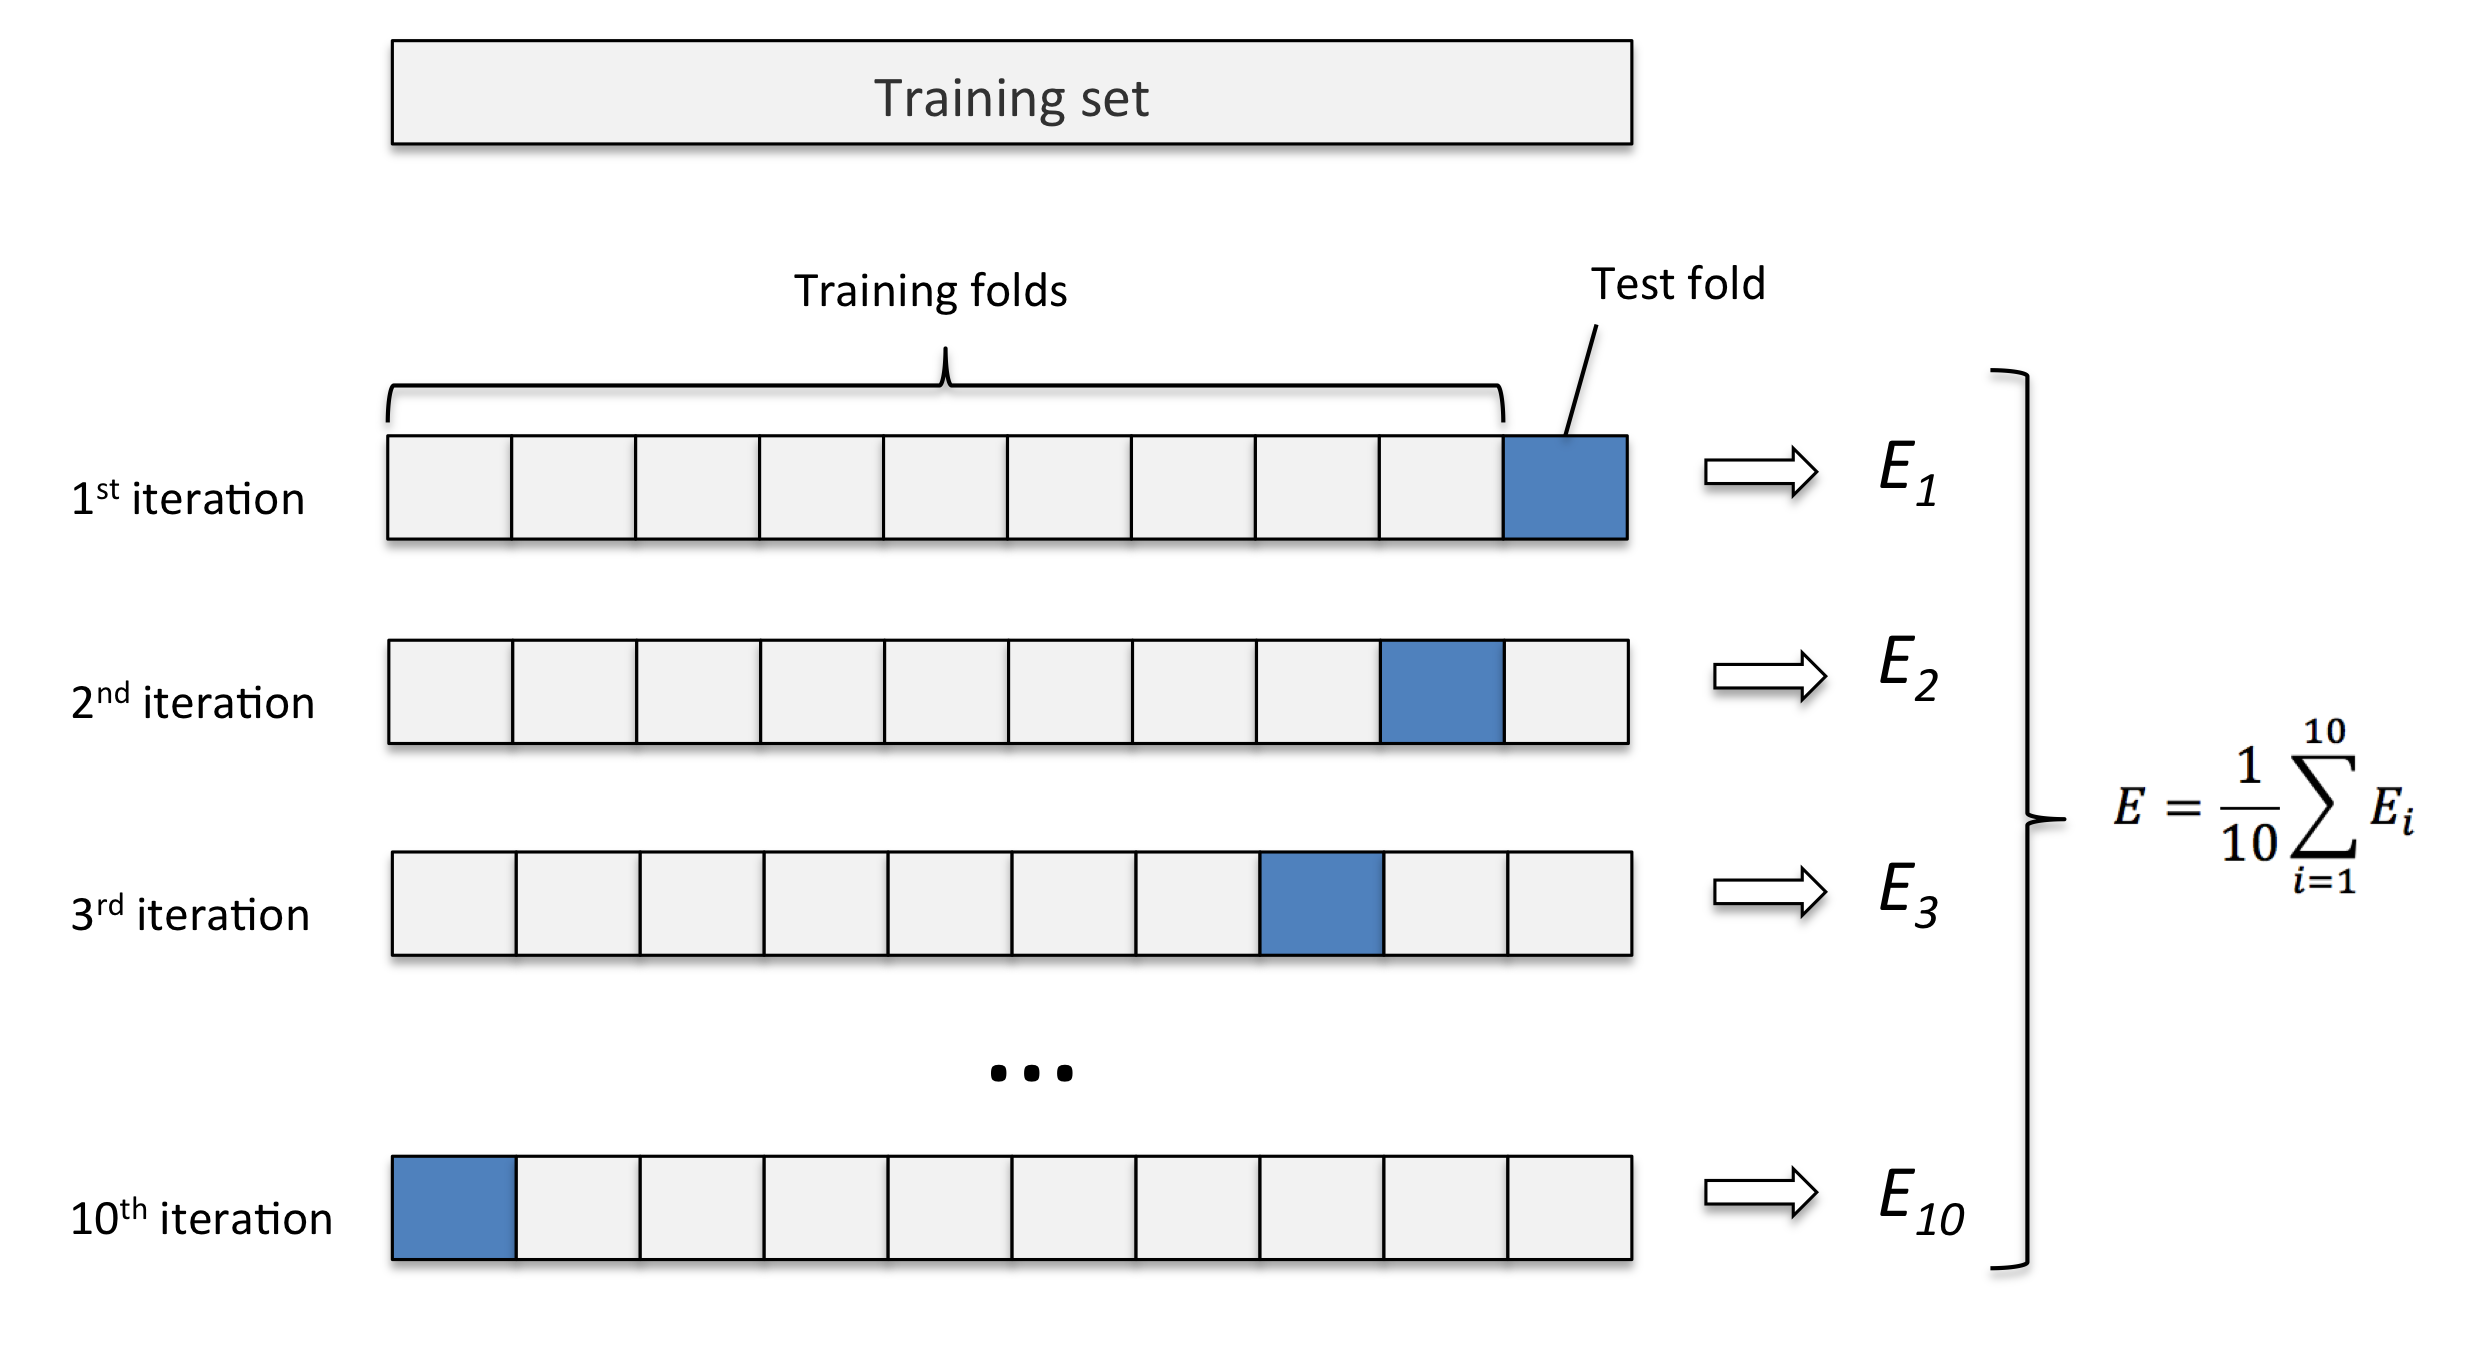
\includegraphics[width=\textwidth]{imagenes/chapter5/cross-validation}
 \end{center}
 \caption{Ejemplo de uso de K-fold para la búsqueda de hiper parámetros.}
 \label{fig:K-fold}
\end{figure}

\subsection{Método con SVM}
Para replicar el método de Zhang et al\cite{NR3DQA} podemos utilizar los 
scripts en \code{NR3DQA/}. Para ello disponemos de unos cuántos scripts para la extracción de las características y visualización de las distribuciones 
como indica la publicación. 
Utilizaremos la librería de Pyntcloud para obtener 
la matriz de covarianza y calcular las características en base a lo definido 
en la Sección \ref{sec:NR3DQA}.
Para los conjuntos de datos SJTU\cite{SJTU} y WPC\cite{WPC1,WPC2}, los resultados 
son similares a los obtenidos en la publicación original, ver Table\ref{tab:PlainNR3DQA}.
Hay que tener en cuenta que para ambos se realiza un K-fold, donde el número 
K es igual al número de nubes de puntos 

\begin{table}[htp]
  \begin{center}
    \begin{tabular}[c]{|c|c|c|c|c|}
      \hline
      \rowcolor[HTML]{FFC702}
      \textbf{Dataset} & \textbf{PLCC} & \textbf{SROCC} & \textbf{KROCC} \\ 
      \hline
      SJTU & 0.810325 & 0.777403 & 0.608302 \\ 
      \hline 
      WPC & 0.637953 & 0.634853 & 0.463578 \\
      \hline
    \end{tabular}
  \end{center}
  \caption[Resultados de prueba preliminar con SVM.]{Resultados de prueba preliminar con SVM.
  En SJTU tenemos una mejora de 7\% que podemos asociar al ruido de la inicialización aleatoria. }
  \label{tab:PlainNR3DQA}
\end{table}

No obstante, utilizando las mismas funciones para el caso de los imágenes médicas 
y experimentando con múltiples modelos de regresión, 
vemos, en la Tabla \ref{tab:MedicalNR3DQA}, que el método no es capaz del todo 
de determinar con precisión la calidad de imágenes, ya que la correlación entre 
la predicción y el valor real es muy cercano a 0. 

\begin{table}[htp]
  \begin{center}
    \hspace{-.5cm}
    \begin{tabular}[c]{|c|c|c|c|c|}
      \hline
      \rowcolor[HTML]{FFC702}
      \multicolumn{1}{|c|}{\textbf{Etiqueta Sintética}} & 
      \multicolumn{1}{|c|}{\textbf{Modelo}} & 
      \multicolumn{1}{|c|}{\textbf{Escalado}} & 
      \multicolumn{1}{|c|}{\textbf{PLCC}} &
      \multicolumn{1}{|c|}{\textbf{SROCC}} \\
      \hline
      Valor de la métrica & SVM & RobustScaler & 0.2017 & 0.1776 \\
      \hline
      Valor normalizado & KNNRegressor & RobustScaler & 0.2671 & 0.1882  \\
      \hline
      Valor en escala 0-5 & DecisionTree & StandardScaler & 0.309176 & 0.196713 \\
      \hline
    \end{tabular}
  \end{center}
  \caption[Resultados de prueba preliminar con SVM.]{Resultados de prueba preliminar con SVM. 
  Vemos los mejores modelos y normalización para las diferentes escalas de las etiquetas sintéticas. 
  Se observa que con el conjunto de imágenes médicas no hemos logrado buena correlación entre 
  los valores predecidos y el valor real.}
  \label{tab:MedicalNR3DQA}
\end{table}

Incluso utilizando el conjunto SJTU\cite{SJTU} para ayudar al entrenamiento 
del SVM, no obtenemos mejoras significativas, sino que obtenemos un 0.225 de SROCC.
Algo similar ocurre cuando intentamos utilizar más características geométricas
como se indica en la publicación\cite{3DNSSMetrics}. Se argumenta que, en el proceso de segmentación, 
detección y clasificación de estructuras en nubes de puntos, 
las mejores métricas suelen ser: 
omnivarianza, entropía de valores singulares, la verticalidad del vecindario y 
otras. Los resultados de utilizar estas métricas adicionales, que 
se pueden observar en la Tabla \ref{tab:ImprovNR3DQA}, no son significativos.

\begin{table}[htp]
  \begin{center}
    \begin{tabular}[c]{|c|c|c|c|c|}
      \hline
      \rowcolor[HTML]{FFC702}
      \textbf{Dataset} & \textbf{PLCC} & \textbf{SROCC} & \textbf{KROCC} \\ 
      \hline
      SJTU & 0.853709 & 0.820057 & 0.649406 \\ 
      \hline 
      WPC & 0.642356 & 0.62917 & 0.455562 \\
      \hline 
      Nuestro & 0.344601 &  0.170793 & -- \\
      \hline
    \end{tabular}
  \end{center}
  \caption[Resultado de mejores sobre el método SVM]{Resultado de mejores sobre el método SVM.
   Se observa mejoras, no sustanciales, sobre los conjuntos SJTU\cite{SJTU}, WPC\cite{WPC1, WPC2} e imágenes médicas.
   No obstante, todavía sigue por detrás de los métodos DL, como el método VQA-PC 
   que se discutirá más adelante.
  }
  \label{tab:ImprovNR3DQA}
\end{table}

En el estado del arte vimos que hay cierta inclinación al uso de modelos 
DL para intentar superar los resultados actuales y obtener una métrica más 
genérica. Se observa la dificultad del análisis de NSS a la hora de elegir que métricas 
deben extraerse para generar un buen vector características para un modelo ML 
que intenta resolver este problema. Dado el marco temporal y visto los 
resultados preliminares de la Sección \ref{sec:PreResults}, se determina 
conveniente hacer uso de modelos más complejos y permitir que la extracción 
de características sea automática. 

\subsection{Experimentos Preliminares DL}
\label{sec:PreResults}
Previo a tratar con los datos médicos, se han realizado pruebas de ejecución 
para verificar el funcionamiento del modelo, validar los resultados, familiarizarse c
on el código e identificar zonas de posibles mejoras.

\subsubsection{Replicando los resultados sobre SJTU}
Para validar el correcto funcionamiento del código y los resultados obtenidos 
en \cite{VQA-PC}, seguimos el experimento en las mismas condiciones descrita 
por ellos en el conjunto de datos SJTU\cite{SJTU}. Como ese posee 10 modelos, 
ver Sección \ref{sec:DatosPublicos}, se realiza un 9-fold. Se ha utilizado 
los mismos hiper parámetros, estructura de red convolucional y transformaciones 
de aumentación de datos, ver Tablas 
\ref{tab:ResNet50} y \ref{tab:HiperSJTU}. 

\begin{table}[htp]
  \begin{center}
    \begin{tabular}[c]{|c|c|}
      \hline
      \rowcolor[HTML]{FFC702}
      \textbf{Hiperparámetro} & \textbf{Valor} \\ 
      \hline 
      Tasa de aprendizaje &  0.0004 \\ 
      \hline 
      Tamaño de batches & 32 \\ 
      \hline 
      Tasa de decadencia & 0.9 \\ 
      \hline 
      Frecuencia de decadencia & 10 \\ 
      \hline 
      Épocas & 30 \\ 
      \hline 
      K-fold & 9 \\ 
      \hline 
    \end{tabular}
  \end{center}
  \caption[Hiper parámetros de prueba preliminar.]{Hiper parámetros de prueba preliminar, establecidos por \cite{VQA-PC}.}
  \label{tab:HiperSJTU}
\end{table}

Para el conjunto de entrenamiento se recorta una zona aleatoria de la imagen con 
tamaño 224x224, a continuación se normaliza los colores conforme al siguiente 
vector de medias $\mu = \left[ 0.485, 0.456, 0.406 \right]$ y de desviación 
$\sigma = \left[ 0.229, 0.224, 0.225 \right]$. Valores con los cuales se 
normalizaron las imágenes con las que entrenó ResNet\cite{ResNet}.
Para el conjunto de test, se utiliza la misma normalización de colores, pero 
en vez de recortar una zona aleatoria de la imagen se recorta la parte central. 

\bgroup
\begin{table}[htp]
  \scriptsize
  \begin{center}
    % \[\setcellgapes{5pt}\makegapedcells % <--- for vertical space around cells contents
    \begin{tabular}[b]{|c|c|c|}
      \hline
      \rowcolor[HTML]{FFC702}
      \multicolumn{1}{|c|}{\textbf{Capa}} & \multicolumn{1}{c|}{\textbf{Salida}}  &
      \multicolumn{1}{c|}{\textbf{Estructura}} \\
      \hline
      Bloque inicial & $112\times112$ & $7\times7,\; 64$, stride 2 \\ 
      \hline 
      \multirow{2}{*}{Bloque convolucional 1} & \multirow{2}{*}{$56\times56$} & $3\times3$ max pool, stride 2 \\ 
      \cline{3-3}
                                              & & $\begin{bmatrix}1\times1,\; 64 \\ 3\times3,\; 64 \\ 1\times1,\; 256 \end{bmatrix}\times 3$ \\ 
      \hline
      Bloque convolucional 2 & $28\times28$ & $\begin{bmatrix}1\times1,\; 128 \\ 3\times3,\; 128 \\ 1\times1,\; 512 \end{bmatrix}  \times 3 $\\ 
      \hline
      Bloque convolucional 3 & $14\times14$ & $\begin{bmatrix}1\times1,\; 256 \\ 3\times3,\; 256 \\ 1\times1,\; 1024 \end{bmatrix} \times 3$ \\ 
      \hline
      Bloque convolucional 4 & $7\times7$   & $\begin{bmatrix}1\times1,\; 512 \\ 3\times3,\; 512 \\ 1\times1,\; 2048 \end{bmatrix}  \times 3 $\\ 
      \hline
      Bloque convolucional 5 & $1\times1$   & average pool, 1000-d fc, softmax\\ 
      \hline
      \multicolumn{2}{|r|}{\cellcolor[HTML]{FFC702}\textbf{Total de parámetros}} & \textbf{23.803.969}\\
      \hline 
      \end{tabular}
    % \]
  \end{center}
  \caption{Descripción de la arquitectura ResNet50\cite{ResNet}.}
  \label{tab:ResNet50}
\end{table}
\egroup

Tras pasada las 9 iteraciones, el resultado promedio es similar al estimado 
por el artículo original y, como se puede observar en la Figura \ref{fig:PreTestCurves},
el modelo parece estar aprendiendo, ver Table \ref{tab:PreTestResults}. 

Se debe tener en cuenta que, aunque el error cuadrático medio pueda parecer 
sustancialmente grande, nuestro criterio de elección sería la correlación 
entre las métricas. Es decir, no necesitamos estimar los valores de distorsión 
en la misma escala que las etiquetas. Apenas necesitamos ser capaces de comparar 
de forma ordenada las imágenes de menor a mayor calidad. En otras palabras, 
si la función a determinar es $f(x) = x$, tener $f(x) = 100x$ sería equivalente.
Por ello, de aquí en adelante utilizaremos la métrica SROCC.

\begin{table}[htp]
  \scriptsize
  \begin{center}
    \begin{tabular}[c]{|c|c|c|}
      \hline
      \rowcolor[HTML]{FFC702}
      \textbf{Kfold} & \textbf{MSE} & \textbf{SROCC} \\ 
      \hline 
      0 & 13.9222 & 0.8995 \\
      \hline 
      1 & 418120.5625 & 0.8547 \\ 
      \hline 
      2 & 10.9271 & 0.9081 \\
      \hline 
      3 & 19.8226 & 0.9295 \\ 
      \hline 
      4 & 443.6077 & 0.8700 \\ 
      \hline 
      5 & 28.3165 & 0.9544 \\ 
      \hline 
      6 & 292.239 & 0.7675 \\ 
      \hline 
      7 & 329.0685 & 0.8833 \\ 
      \hline 
      8 & 357.0455 & 0.8647 \\ 
      \hline
      \textbf{\cellcolor[HTML]{FFC702}Promedio} & \textbf{46623.94} & \textbf{0.8813} \\ 
      \hline
    \end{tabular}
  \end{center}
  \caption[Resultados de experimento preliminar.]{Resultados de experimento preliminar. 
    Cabe observar que los valores se acercan a los resultados obtenidos en la publicación original, 
    utilizando el criterio del promedio del mejor resultado de cada pliegue de validación. 
    El error enseñado es el error MSE del modelo, sin utilizar la regresión logística.
}
  \label{tab:PreTestResults}
\end{table}

\begin{figure}[htp]
  \begin{subfigure}[b]{0.49\textwidth}
  \centering
    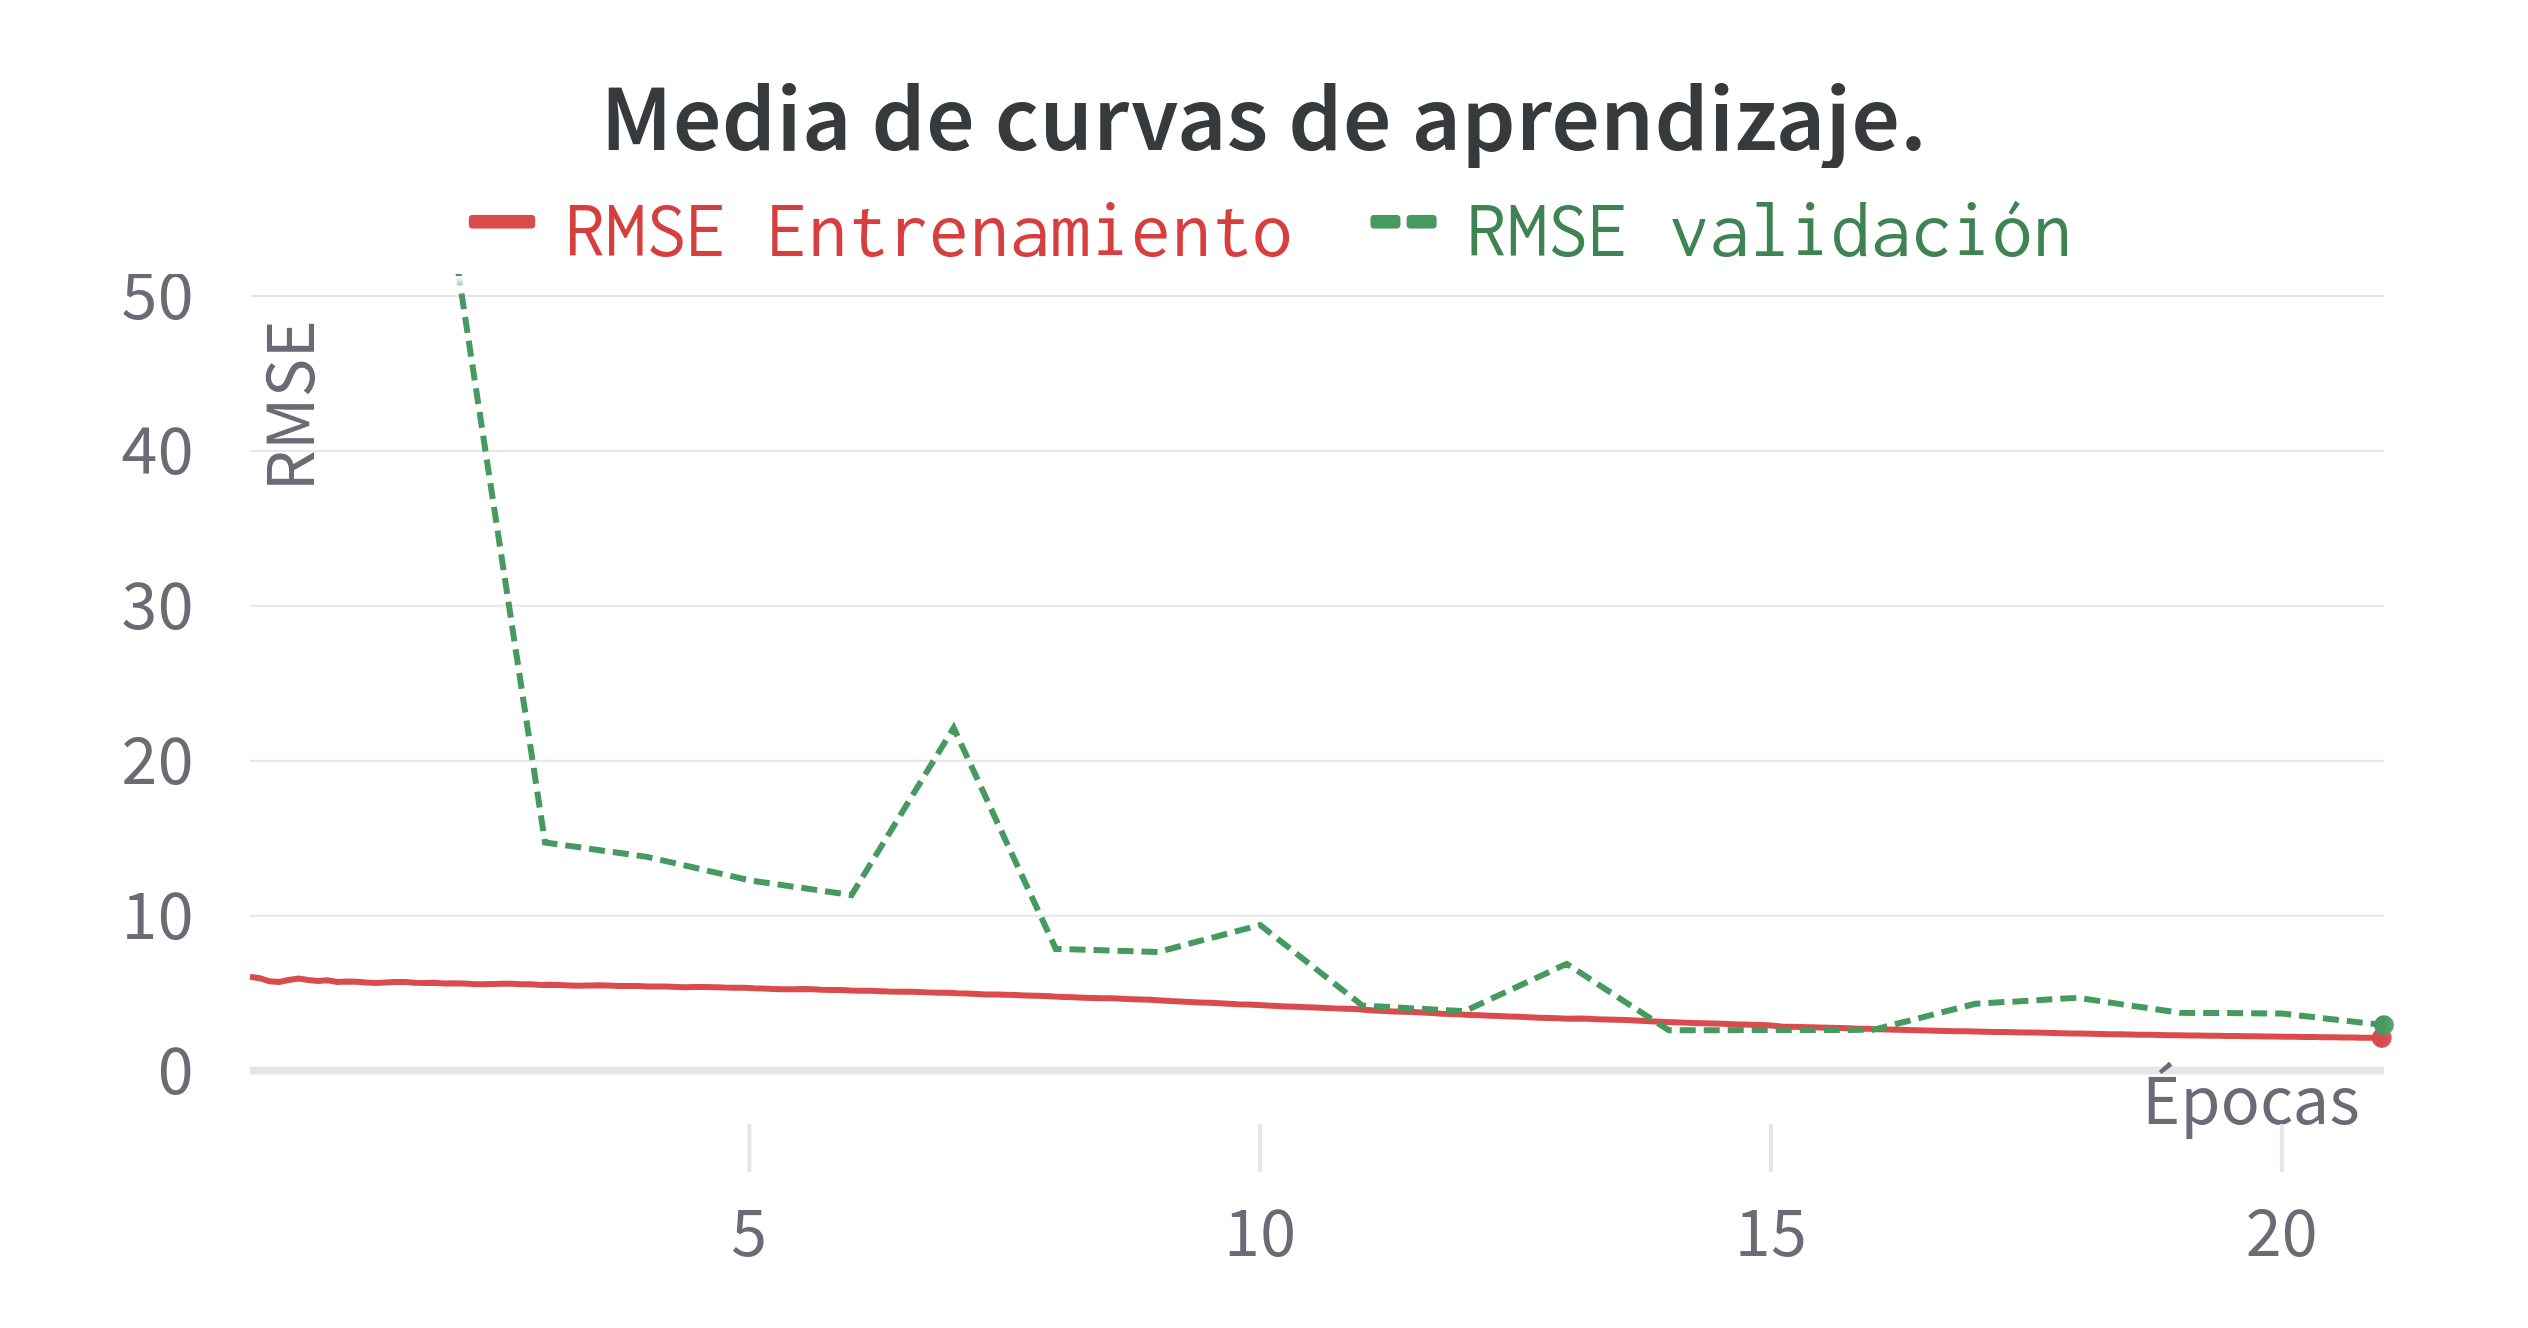
\includegraphics[width=\textwidth]{imagenes/chapter5/PreTestCurves.png}
  \end{subfigure}
  \begin{subfigure}[b]{0.49\textwidth}
  \centering
    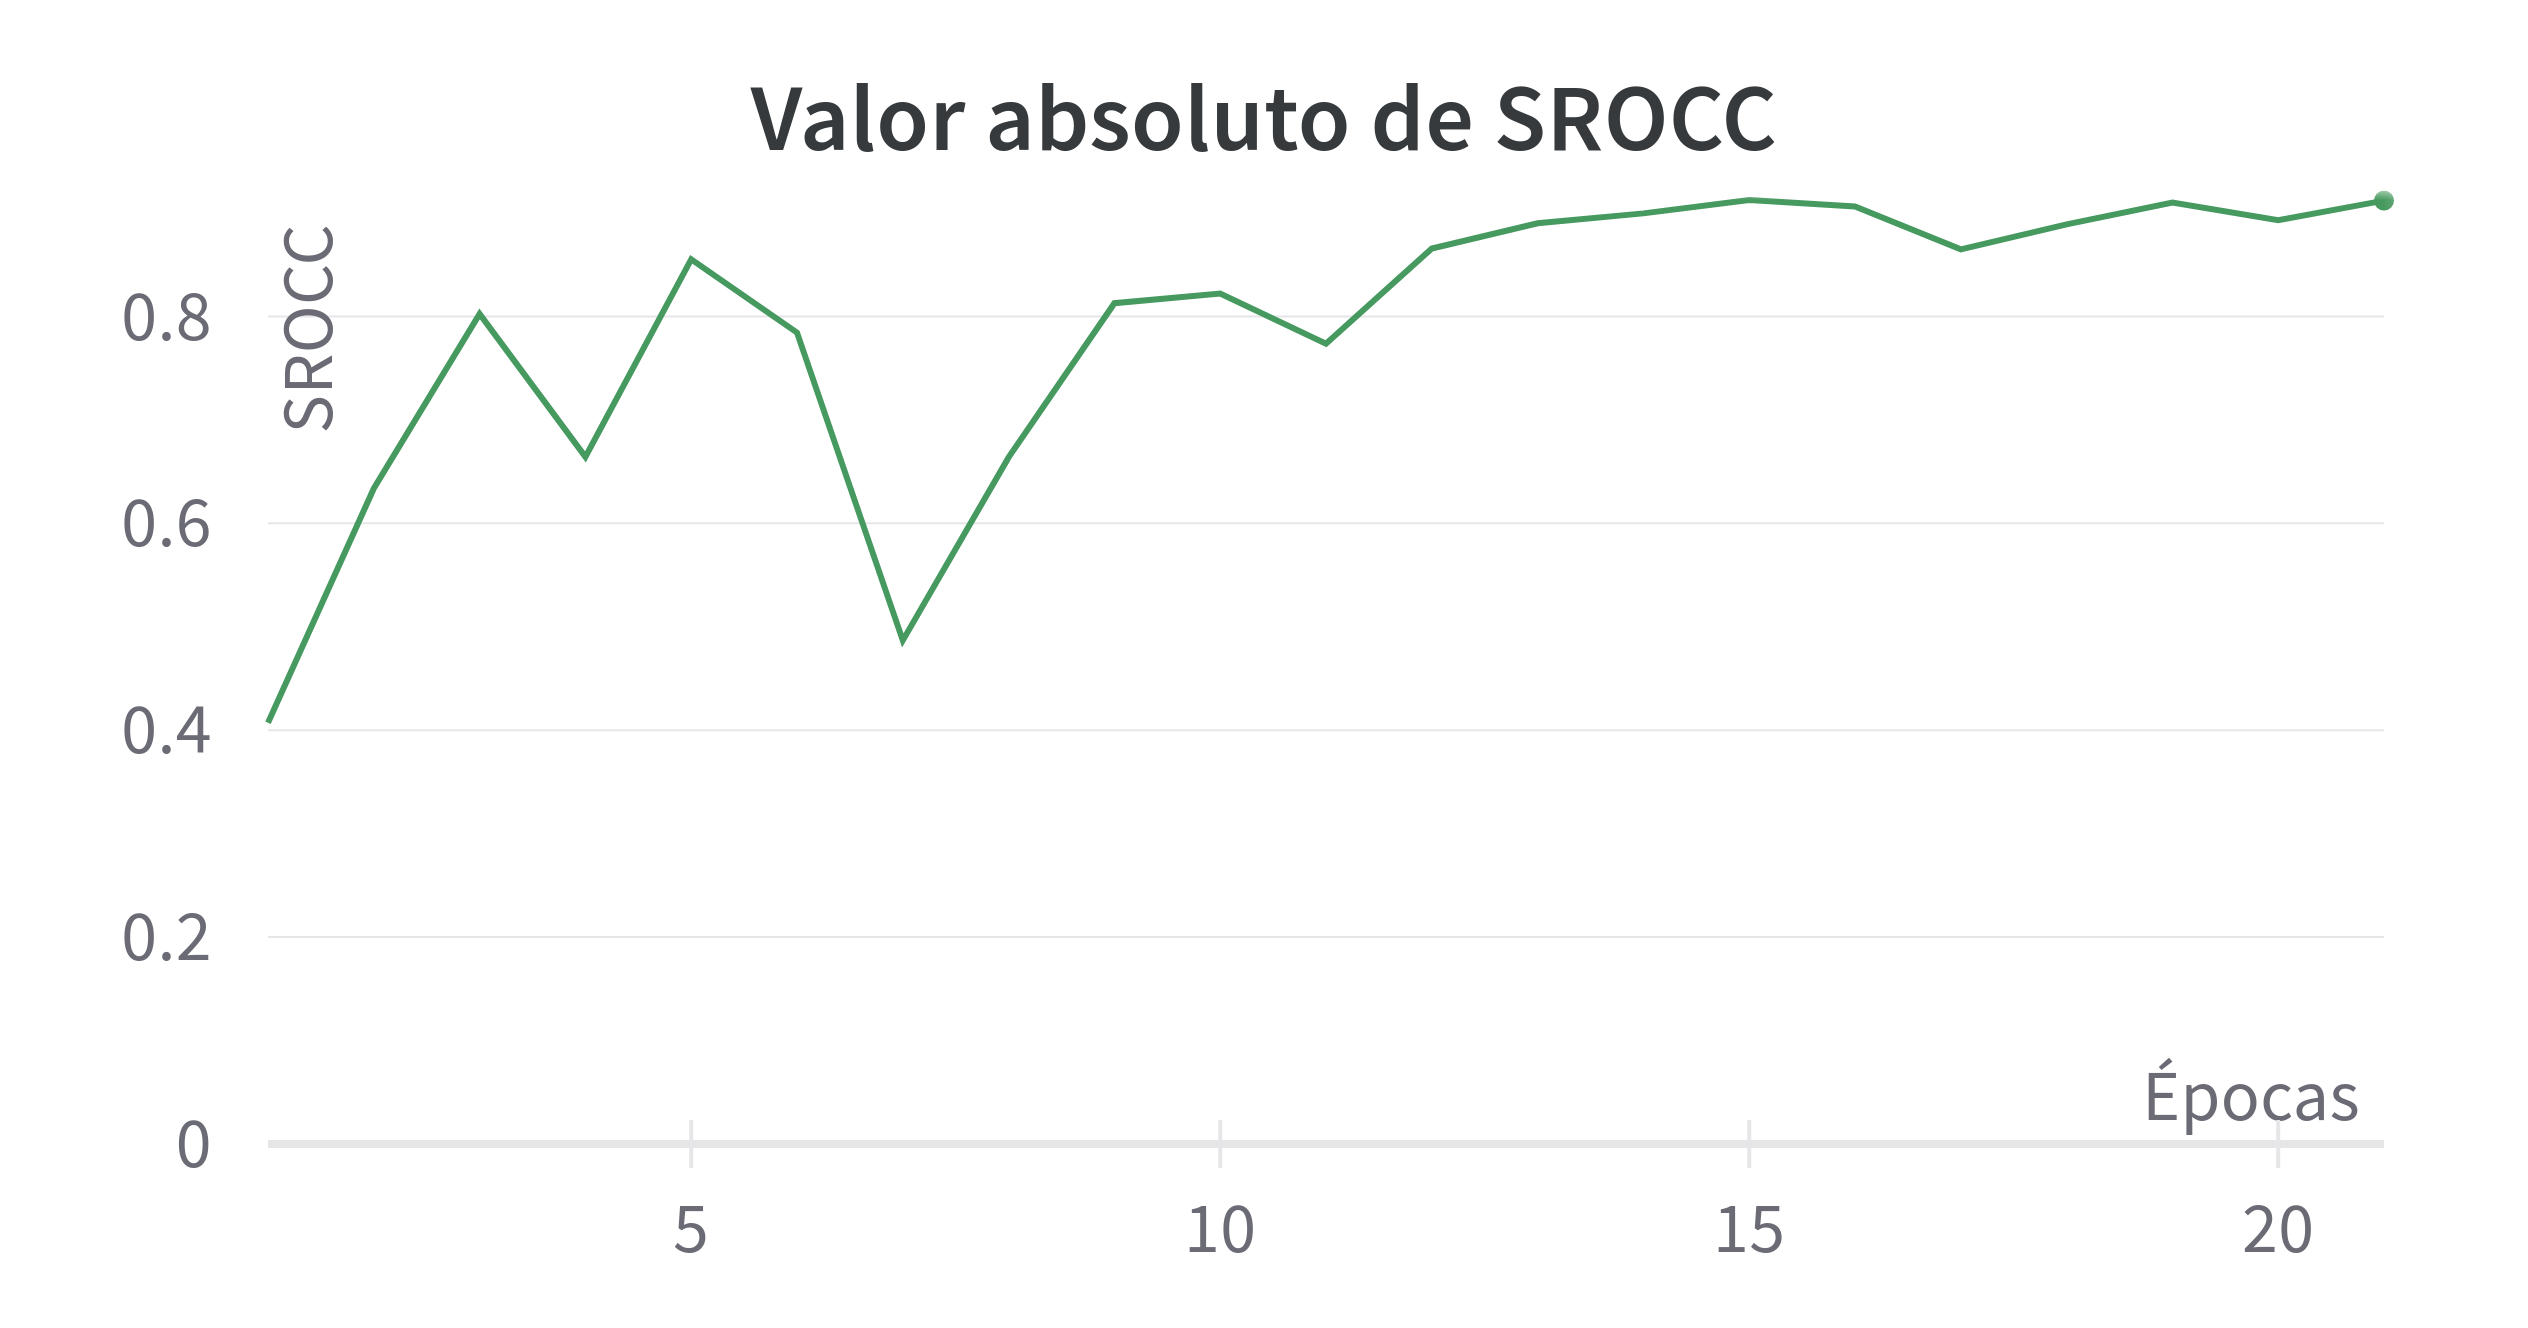
\includegraphics[width=\textwidth]{imagenes/chapter5/PreTestSROCC.png}
  \end{subfigure}
  \caption[Curvas de aprendizaje del test preliminar.]{Curvas de aprendizaje del test preliminar. Es el comportamiento medio en cada fold.
  Como vemos el error de validación tiende a bajar, aunque con cierta variabilidad 
  entre épocas en contra del error de entrenamiento que es más estable. A la derecha 
  podemos ver el comportamiento de la métrica SROCC en valor absoluto 
  (resolver el problema inverso sería equivalente).}
  \label{fig:PreTestCurves}
\end{figure}


\subsection{Propuestas de mejoras}
La publicación \cite{EnsemblePCQA} propone distintos métodos para la fusión de vectores características de modelos \emph{ensemble}.
En ella, se realiza una comparativa entre cuatro métodos: la concatenación, multiplicación, convolución 1x1 y 
fusión en el dominio de fourier. 
Argumenta que cada uno de los métodos de fusión permite la interacción de los vectores 
características de distinta manera. El método de concatenación, aunque es el método 
más habitual, genera vectores de mayor dimensionalidad, hecho que puede influir 
sustancialmente al tiempo de entrenamiento e inferencia. Además, no permite una interacción directa entre los vectores. 
Es por ello que se experimenta con los demás métodos.  

La fusión por multiplicación (F1) puede provocar pérdida de información (valores cercanos a 0). 
No obstante, permiten una interacción directa de los vectores y genera un vector salida 
de menor dimensionalidad. Otro inconveniente es que tenemos normalizar, si no son 
ya iguales, a la misma dimensión los vectores. De forma similar, la fusión por convolución (F2)
permite realizar una proyección lineal de ambos vectores a uno de menor dimensionalidad. 
Por último, la fusión por \emph{bi-linear pooling} (F3) permite realizar la multiplicación de 
los vectores en el dominio de fourier, de tal forma que todos los elementos afectan al 
resultado final de forma multiplicativa sin un alto coste computacional, y luego proyecta 
el vector resultante a una menor dimensión utilizando algún algoritmo de proyección, 
como \emph{Count Sketch}. Se han utilizado los mismos hiperparámetros que definido 
en la Tabla \ref{tab:HiperSJTU}.

Por último, se observa que el modelo realiza un recorte aleatorio de las imágenes de entrada, 
originalmente a escala 1920x1080, durante el entrenamiento 
para ajustarlas a una escala de 224x224, lo cual reduce el tiempo de cómputo y 
evita el sobre-entrenamiento. Durante la ejecución del test, se recorta el centro de la imagen. 
Este proceso de rescalado, conocido como aumentación de datos, incrementa la cantidad de ejemplos 
y previene el sobreajuste. Sin embargo, debido a que las nubes de puntos ocupan principalmente 
la zona central de la imagen y poca proporción, se propone un rescalado uniforme a una escala de 
398x224 para obtener recortes válidos y relevantes.

Para realizar la comparativa de estas mejoras, se utiliza el conjunto de datos 
médicos definidos anteriormente. Se hace la comparativa con las métricas sin 
normalizar y normalizadas a la escala 0-5, la misma con la que se entrenó VQA-PC\cite{VQA-PC} en SJTU\cite{SJTU}. 
Se entrena por 30 épocas, con el uso de \emph{early-stopping}, método utilizado para frenar el entrenamiento 
si el error de validación crece para evitar sobre-entrenamiento, con una paciencia 
de 6 épocas (en este contexto, paciencia alude a la espera de los resultados de 
las N siguientes épocas, en la que el error de validación crece, antes de terminar 
la ejecución por sobre-entrenamiento). 

\begin{table}[htp]
  \scriptsize
  \centering
\begin{tabular}{|c|cccc|}
\hline
\rowcolor[HTML]{FFC702}
                       & \multicolumn{4}{c|}{\textbf{Valor medio SROCC}}                                                                                                    \\ \hline
\rowcolor[HTML]{FFC702}
\textbf{Modelo}        & \multicolumn{1}{c|}{\textbf{Estándar}} & \multicolumn{1}{c|}{\textbf{Normalizado}} & \multicolumn{1}{c|}{\textbf{Rescalado}} & \textbf{Ambos}  \\ \hline
\textbf{VQA-PC (SJTU)} & \multicolumn{1}{c|}{0.7094}            & \multicolumn{1}{c|}{\textbf{0.6235}}      & \multicolumn{1}{c|}{\textbf{0.8425}}    & 0.7126          \\ \hline
\textbf{VQA-PC F1}     & \multicolumn{1}{c|}{\textbf{0.7305}}   & \multicolumn{1}{c|}{0.6140}               & \multicolumn{1}{c|}{0.8164}             & 0.7291          \\ \hline
\textbf{VQA-PC F2}     & \multicolumn{1}{c|}{0.6816}            & \multicolumn{1}{c|}{0.5770}               & \multicolumn{1}{c|}{0.8057}             & \textbf{0.7324} \\ \hline
\textbf{VQA-PC F3}     & \multicolumn{1}{c|}{0.7080}            & \multicolumn{1}{c|}{0.5671}      & \multicolumn{1}{c|}{0.7482}             & 0.7006          \\ \hline
\end{tabular}
\caption[Valor medio sobre imágenes médicas.]{Tabla de resultados iniciales sobre imágenes médicas. 
Partimos del modelo pre-entrenado de la publicación original \cite{VQA-PC} sobre SJTU\cite{SJTU}. Hacemos 
11-fold sobre nuestro conjunto de datos teniendo en cuenta las métricas originales, las métricas
normalizadas a escala 0-5 y las imaǵenes rescaladas. También se investiga rescalar y normalizar (última columna).
Se compara estos resultados con los demás métodos de fusión de características propuesto.
Vemos que el modelo con información previa, al utilizar el rescalado, obtiene los mejores resultados.
No obstante, F1 y F2 sin información previa consiguen acercarse a un margen de 4\% de ese valor. 
Por otro lado, la fusión F3 no logra mejorar de forma significativas los resultados. 
}
\end{table}

Los resultados son prometedores. El modelo con información adicional sobre otros 
tipos de distorsiones, conocimiento del conjunto SJTU, es el que obtiene el mejor 
resultado tras rescalar las imágenes, seguido por el modelo entrenado desde 0 
con la fusión por multiplicación (F1). No obstante, se ha observado cierta 
variabilidad en los resultados de cada pliegue, como se observa en la Tabla \ref{tab:STDevMed}.
Esto puede ser debido a diversos factores, desde la dificultad del modelo de 
aprender las características relevantes en tan pocas épocas, por la falta 
de ejemplos en este pequeño conjunto de imágenes médicas, por la variabilidad 
entre nubes de puntos (pocos ejemplos similares y muchas partes del cuerpo) 
o por dificultades en la generación de etiquetas sintéticas de calidad. 
Además, observándose detenidamente los valores obtenidos en cada pliegue, 
se observa una alta variabilidad para un ejemplo en concreto, el último pliegue, 
con SROCC a más de 3 desviaciones típicas para los casos F1-F3.  Es por ello, 
que se puede observar la mediana de cada modelo en la Tabla \ref{tab:PercentileMed}.

Para validar el rápido aprendizaje de los métodos F1-F3 y la posible mejora 
sobre el método de concatenación, se experimenta utilizar el modelo VQA-PC sin 
modificaciones desde 0 sobre las imágenes rescaladas, ver Tabla \ref{tab:VQAF0}.
Se determina que las mejoras F1-F3 no son significativas sin información adicional. 
Dado la importancia de la información adicional sobre las distorsiones a la 
hora de estimar la calidad de las imágenes de nuestro pequeño conjunto médico, 
se propone pre-entrenar sobre el conjunto LS-SJTU-PCQA\cite{ResSCNN}.
En este caso, se utilizará las imaǵenes rescaladas y las métricas sin normalizar, 
dado que se ha observado anteriormente que es la mejor combinación.
Se observa una mejora significativa en el método F3, y se logra 
pasar la barrera del 90\% en la mediana del método F0, ver Tabla \ref{tab:LS-SJTU-FN}.

\begin{table}[htp]
  \scriptsize
  \centering
\begin{tabular}{|c|cccc|}
\hline
\rowcolor[HTML]{FFC702}
                       & \multicolumn{4}{c|}{\textbf{Desviación típica SROCC}}                                                                                                \\ \hline
\rowcolor[HTML]{FFC702}
\textbf{Modelo}        & \multicolumn{1}{c|}{\textbf{Estándar}} & \multicolumn{1}{c|}{\textbf{Normalizado}} & \multicolumn{1}{c|}{\textbf{Rescalado}} & \textbf{Ambos}  \\ \hline
\textbf{VQA-PC (SJTU)} & \multicolumn{1}{c|}{0.1448}            & \multicolumn{1}{c|}{0.2357}               & \multicolumn{1}{c|}{\textbf{0.0668}}    & 0.1335          \\ \hline
\textbf{VQA-PC F1}     & \multicolumn{1}{c|}{\textbf{0.1222}}   & \multicolumn{1}{c|}{0.1402}               & \multicolumn{1}{c|}{0.1752}             & 0.2250          \\ \hline
\textbf{VQA-PC F2}     & \multicolumn{1}{c|}{0.1462}            & \multicolumn{1}{c|}{0.1905}               & \multicolumn{1}{c|}{0.1741}             & \textbf{0.1187} \\ \hline
\textbf{VQA-PC F3}     & \multicolumn{1}{c|}{0.1507}            & \multicolumn{1}{c|}{\textbf{0.1304}}      & \multicolumn{1}{c|}{0.1326}             & 0.1462          \\ \hline
\end{tabular}
\caption[Desviación típica de los resultados médicos]{Desviación típica de los 
resultados obtenidos. Se observa que la mejora del rescalado de las imágenes 
de entrada mejora la estabilidad del modelo inicial. El método de fusión F3 
es el más estable en todos los casos. }
\label{tab:STDevMed}
\end{table}

\begin{table}[htp]
  \scriptsize
  \centering
\begin{tabular}{|c|cccc|}
\hline
\rowcolor[HTML]{FFC702}
                       & \multicolumn{4}{c|}{\textbf{Mediana SROCC}}                                                                                                          \\ \hline
\rowcolor[HTML]{FFC702}
\textbf{Modelo}        & \multicolumn{1}{c|}{\textbf{Estándar}} & \multicolumn{1}{c|}{\textbf{Normalizado}} & \multicolumn{1}{c|}{\textbf{Rescalado}} & \textbf{Ambos}  \\ \hline
\textbf{VQA-PC (SJTU)} & \multicolumn{1}{c|}{\textbf{0.7400}}   & \multicolumn{1}{c|}{\textbf{0.7510}}      & \multicolumn{1}{c|}{0.8417}             & 0.7434          \\ \hline
\textbf{VQA-PC F1}     & \multicolumn{1}{c|}{0.7022}            & \multicolumn{1}{c|}{0.6331}               & \multicolumn{1}{c|}{\textbf{0.8636}}    & \textbf{0.7849} \\ \hline
\textbf{VQA-PC F2}     & \multicolumn{1}{c|}{0.6350}            & \multicolumn{1}{c|}{0.5955}               & \multicolumn{1}{c|}{0.8538}             & 0.7165          \\ \hline
\textbf{VQA-PC F3}     & \multicolumn{1}{c|}{0.7118}            & \multicolumn{1}{c|}{0.5179}               & \multicolumn{1}{c|}{0.7518}             & 0.7334          \\ \hline
\end{tabular}
\caption[Mediana de los valores sobre imágenes médicas.]{
  Mediana de los valores obtenidos. Se observa una mejora significativa para 
  los métodos F1 y F2. También es evidente la estabilidad del modelo pre-entrenado
  sobre SJTU\cite{SJTU}. 
}
\label{tab:PercentileMed}
\end{table}


\begin{table}[htp] 
  \scriptsize
  \centering
  \begin{tabular}{|c|c|c|c|}
\hline
\rowcolor[HTML]{FFC702}
                       & \multicolumn{3}{c|}{\textbf{SROCC}}                                                                                                          \\ \hline
\rowcolor[HTML]{FFC702}
\textbf{Modelo}        & \multicolumn{1}{c|}{\textbf{Media}} & \multicolumn{1}{c|}{\textbf{Desviación}} & \multicolumn{1}{c|}{\textbf{Mediana}} \\ \hline
\textbf{VQA-PC F0} & \multicolumn{1}{c|}{\textbf{0.8261}}   & \multicolumn{1}{c|}{0.1589}      & \multicolumn{1}{c|}{\textbf{0.8657}}      \\ \hline
  \end{tabular}
  \caption[Resultados del método original sin pre-entrenar sobre imágenes rescaladas.]{
    Resultados del método original sin pre-entrenar sobre imágenes rescaladas. 
    Se obtiene resultados, en media, algo peor que el modelo 
  pre-entrenado, remarcando la importancia de información adicional y etapas 
  de entrenamiento más largas a la hora de lidiar con algunas nubes de puntos, y 
  en mediana se obtiene el mejor resultado. De esta forma, para un conjunto 
  de datos pequeños se descarta el uso de las mejoras F1-F3.
}
\label{tab:VQAF0}
\end{table}
\begin{table}[htp]
  \scriptsize
  \centering
\begin{tabular}{|c|c|c|c|}
  \hline
\rowcolor[HTML]{FFC702}
                       & \multicolumn{3}{c|}{\textbf{SROCC}} \\ \hline
\rowcolor[HTML]{FFC702}
\textbf{Modelo}    & \textbf{Media} & \textbf{Desviación} & \textbf{Mediana}   \\ \hline
\textbf{VQA-PC F0} & 0.7980           & 0.2332              & \textbf{0.9258}    \\ \hline
\textbf{VQA-PC F1} & 0.7378           & 0.2265              & 0.8322             \\ \hline
\textbf{VQA-PC F2} & 0.8354           & \textbf{0.1040}     & 0.8370             \\ \hline
\textbf{VQA-PC F3} & \textbf{0.8605}  & 0.1104              & 0.8824             \\ \hline
\end{tabular}
\caption[Resultados en imágenes médicas rescaladas entrenando en LS-SJTU-PCQA.]{
  Resultados en imágenes médicas rescaladas entrenando en LS-SJTU-PCQA. 
  Gracias a la información adicional hemos logrado medianas mucho mejores, llegando a 
  obtener una correlación del 92\% con el modelo F0. Sin embargo, en algunos pliegues 
  la información adicional ha empeorado la capacidad del modelo de aprender, con 
  excepción del modelo F3 que en este caso ha logrado obtener la mejor media, un 86\%.
}\label{tab:LS-SJTU-FN}
\end{table}
